\chapter{Negative Pion Cross Section Measurement}

\section{Estimate of $E_{loss}$ before the TPC}
The beamline particles travel a path from when their momentum is measured by the beamline detector, until they are tracked again inside the TPC. In the current LArIAT geometry, a particle leaving the fourth wire chamber will encounter the materials listed in Table \ref{tab:budget} before being registered again. The energy lost by the particle in this non-instrumented material modifies the particle's kinetic energy and directly affects the cross section measurement, as shown in equation \ref{eq:enFF}.

\begin{table}[h!]
\centering
\begin{tabular}{|l|l|l|}
\hline
Material  & density {[}g/cm$^3${]} & width {[}cm{]}    \\ \hline
Fiberglass laminate (G10)      & 1.7                             & 1.28                              \\
Liquid Argon                           & 1.4                             & 3.20                             \\
Stainless Steel                        & 7.7                            & 0.23                             \\
Titanium                                  & 4.5                            & 0.04                             \\ 
Air                                            &  1.2 $\cdot10^{-3}$  & 89.43                              \\
Plastic Scintillator                    & 1.03                          & 1.20 (+ 1.30)                             \\ \hline
\end{tabular}
\caption{LArIAT material budget from WC4 to the TPC Front Face.}
\label{tab:budget}
\end{table}


We derive an estimate of the energy loss between the beamline momentum measurement and the TPC ($E_{loss}$) from the Data Driven Monte Carlo using the pion and kaon samples separately, since this quantity is not  measurable directly on data. 
The $E_{loss}$ distribution for the 60A  and 100A pion sample is shown in figure \ref{fig:ELoss60A}, left and right respectively. A clear double peaked structure is visible, which is due to the particles either missing or hitting the HALO paddle: a schematic rendering of this occurrence is  shown in figure \ref{fig:Halo}. The kinematic at WC4 determines the trajectory of a particle and whether or not it will hit the halo paddle. In figure \ref{fig:PxVsXTrue} , we plot the true  $X$ component of the momentum versus the true $X$ position at WC4 for pions missing the halo paddle (left) and for pions hitting the halo paddle (right) for the 60A MC simulation runs -- analogous plots are obtained with the 100A simulation. These distributions can be separated drawing a line in this position-momentum space. 
We use a logistic regression  \cite{agresti2013categorical}  as a classifier to find the best separating line, shown in both plots as the red line. We classify as ``hitting the halo paddle" all pions whose $P_x$ and $X$ are such that $$P_x +0.02* X - 0.4 < 0 $$ and as ``missing the halo  paddle" all pions whose $P_x$ and $X$ are such that $$P_x +0.02*X - 0.4 > 0, $$ where the coefficients of the line are empirically found by the logistic regression estimation. Overall, this simple classifier classifies in the right category (hit or miss) about 86\% of the pion events.
We apply the same classifier on data. We assign  $E_{loss} = 32 \pm 4 $~MeV for events classified as ``hitting the halo paddle"; we assign  $E_{loss} = 24 \pm 3 $~MeV for events classified as ``missing the halo paddle".

%We use the separation of these two distributions to decide what the energy loss for each event on data. 
%Thus,  we assign the value for energy loss is used in the data.


\begin{figure}[hbpt]
\centering
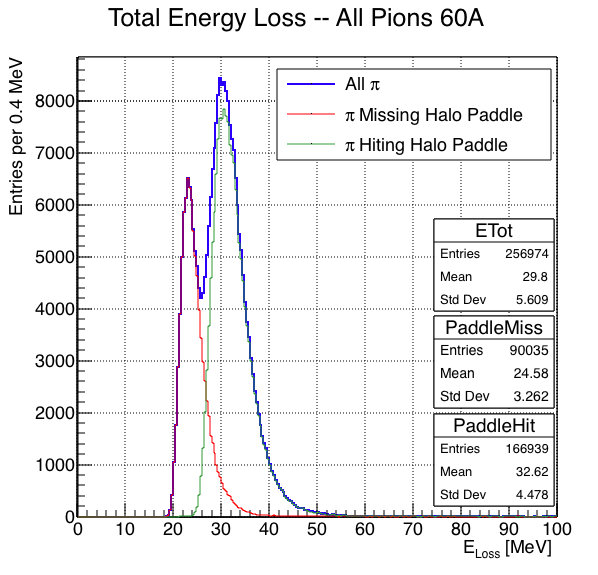
\includegraphics[width=0.45\textwidth]{Chapter-5/Images/E_loss60A.png}
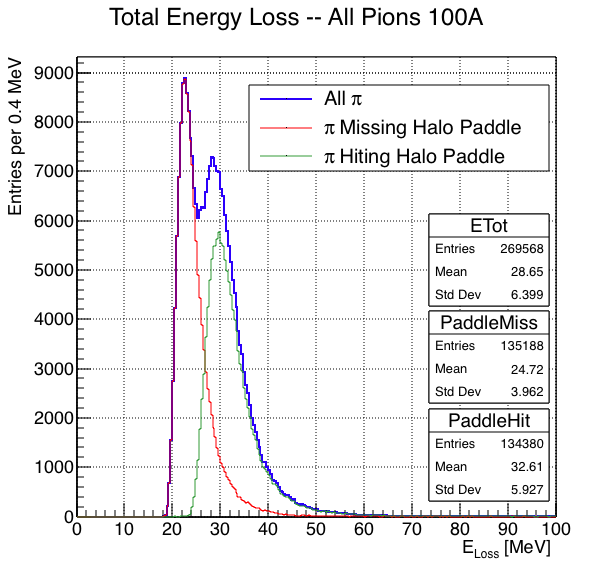
\includegraphics[width=0.45\textwidth]{Chapter-5/Images/E_loss100A.png}
\caption{True energy loss between WC4 and the TPC front face according to the MC simulation of the 60A runs (left) and of the 100A runs (right). The distribution for the whole data sample is shown in blue, the distribution for the pions missing the halo is shown in red, and the distribution for the pions hitting the halo is shown in green.  }
\label{fig:ELoss60A}
\end{figure}

\begin{figure}[hbpt]
\centering
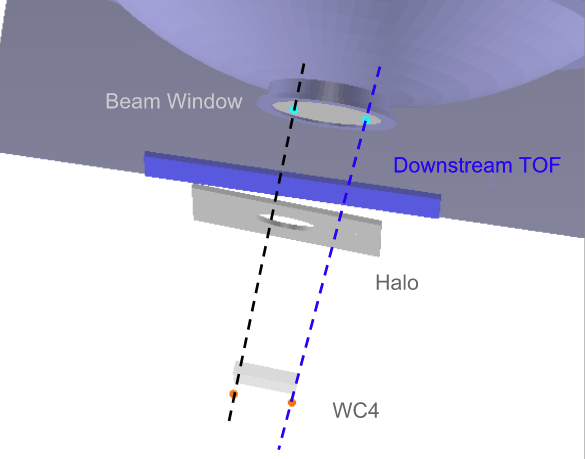
\includegraphics[scale=0.5]{Chapter-5/Images/Halo.png}
\caption{Schematic rendering of the particle path between WC4 and the TPC front face. The paddle with the hollow central circle represents the Halo paddle. We illustrate two possible trajectories: in black, a trajectory that miss the paddle and goes through the hole in the Halo, in blue a trajectory that hits the Halo paddle and goes through the scintillation material.}
\label{fig:Halo}
\end{figure}



\begin{figure}[hbpt]
\centering
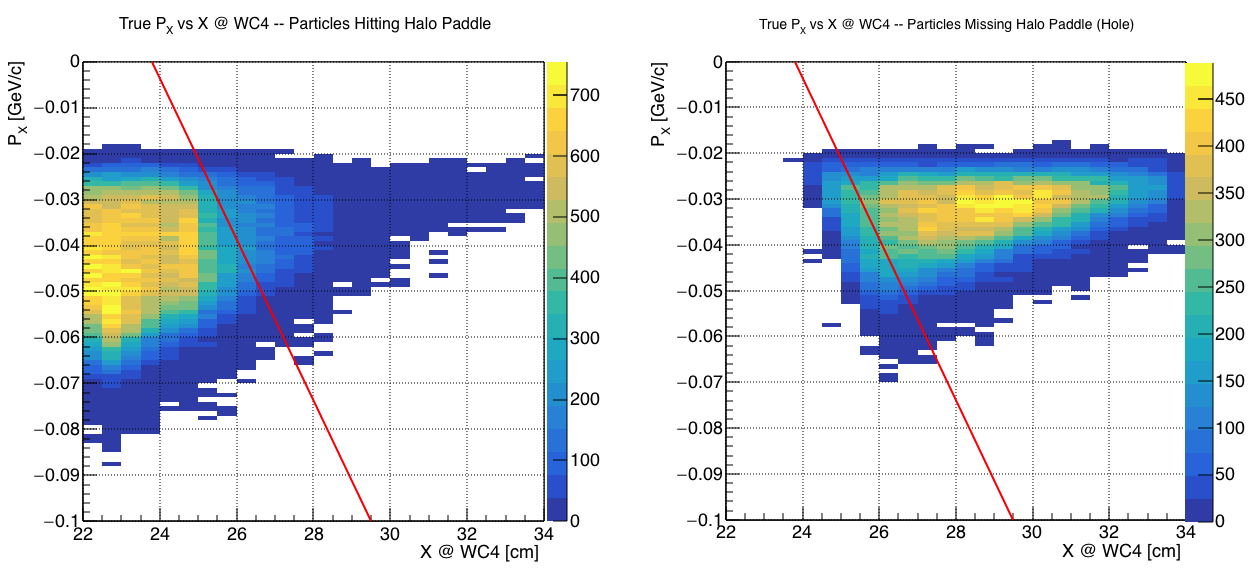
\includegraphics[width=\textwidth]{Chapter-5/Images/PXVsX60A.png}
\caption{Horizontal component of the true momentum vs the horizontal position at WC4 for MC simulated pions of the 60A runs. The plot on the left shows the distribution for pion that miss the halo paddle and the plot on the right shows the distributions for pions that hit the halo. The form of the classifier is overlaid to both plots (red line).}
\label{fig:PxVsXTrue}
\end{figure}

\section{Interacting and Incident Distributions}

\section{Total Hadronic Negative Pion-Argon Differential Cross Section}

